\documentclass[12pt]{scrreprt}

%------------------------------------------------------
% LaTeX packages
%------------------------------------------------------
\usepackage[ngerman]{babel}
\usepackage{pdfpages}
\usepackage{geometry} 
\usepackage{url}
\usepackage{cite}
\usepackage{ae}
\usepackage[ngerman]{babel}          % Umlaute  
\usepackage[ansinew]{inputenc}
\usepackage[T1]{fontenc}
\usepackage{lmodern} 							% neue deutsche Trennungsregeln, etc 
\usepackage{mathptmx} 							% Schriftart (Times New Roman)
\usepackage{acronym}
\usepackage[onehalfspacing]{setspace}	% Eineinhalb Zeilen Abstand
\usepackage{titlesec}
\usepackage{hyperref}
\usepackage{minitoc}
\usepackage{scrpage2}


%------------------------------------------------------
% Glossaries
%------------------------------------------------------
\usepackage[nonumberlist, %keine Seitenzahlen anzeigen
acronym,      %ein Abk�rzungsverzeichnis erstellen
toc,          %Eintr�ge im Inhaltsverzeichnis
section]      %im Inhaltsverzeichnis auf section-Ebene erscheinen
{glossaries} % Glossar

%------------------------------------------------------
% Seitenzahlformatierung (rechts)
%------------------------------------------------------
\pagestyle{plain} 
\cfoot[]{}% [plain-Seiten]{normale Seiten} 
\ofoot[\pagemark]{\pagemark} 

%--------------------------------------------------------------------------- 
% �berschriften 
%--------------------------------------------------------------------------- 
\titleformat{name=\chapter,numberless}[display]{\normalfont\huge\bfseries}{\titlerule}{-7ex}{}[\vspace{5ex}]
\titleformat{\chapter}{\normalfont\huge\bfseries}{\thechapter}{20pt}{\Huge}
\titlespacing{\chapter}{0em}{2.5em}{0em} % {left}{before}{after}[right]
\titleformat{\section}{\normalfont\LARGE\bfseries}{\thesection}{16pt}{\LARGE}
\titleformat{\subsection}{\normalfont\Large\bfseries}{\thesubsection}{14pt}{\Large}
\titleformat{\subsubsection}{\normalfont\large\bfseries}{\thesubsubsection}{14pt}{\large}

%------------------------------------------------------
% Space after Minitoc
%------------------------------------------------------
\mtcsetfeature{minitoc}{close}{\vspace{.5cm}}

%------------------------------------------------------
% Settings
%------------------------------------------------------
\geometry{a4paper, left=30mm, right=25mm, layoutheight=315mm}
% !TEX root = Glossar.tex
\makeglossaries




\newglossaryentry{big_data}
{
	name=Big Data,
	description={Inhalt ....}
}


\newglossaryentry{industrie_4.0}
{
	name=Industrie 4.0,
	description={Inhalt ....}
}


\newglossaryentry{iot}
{
	name=IoT,
	description={Inhalt ....}
}


\newglossaryentry{embedded_systems}
{
	name=Embedded Systems,
	description={Inhalt ....}
}







%------------------------------------------------------
% START OF DOCUMENT
%------------------------------------------------------
\begin{document}

%------------------------------------------------------
% Minitoc settings
%------------------------------------------------------	
\dominitoc
\mtcsettitle{minitoc}{}


%------------------------------------------------------
% Deckblatt & Einverst�ndnisserkl�rung
%------------------------------------------------------

\includepdf[pages={1}]{Deckblatt-BA.pdf}
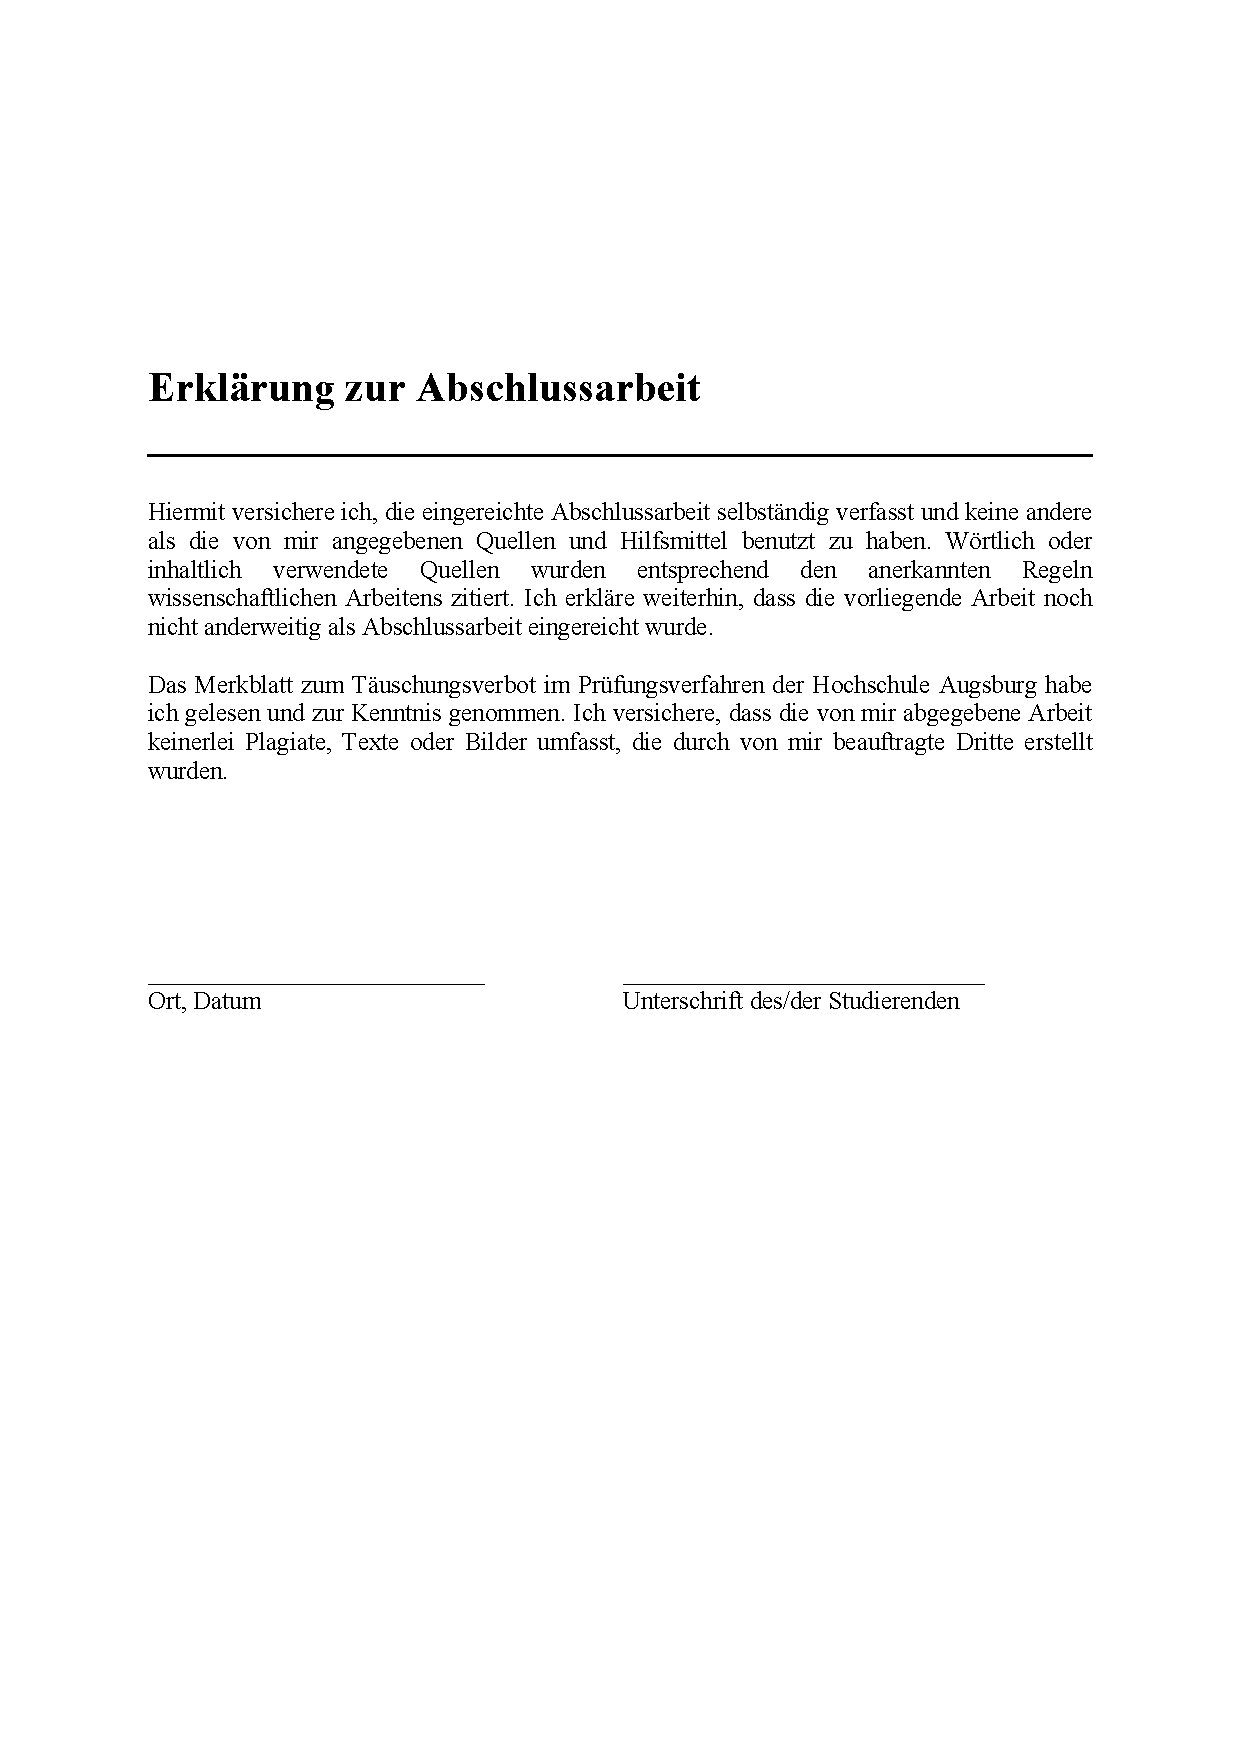
\includepdf[]{Erstellungserklaerung-Abschlussarbeit.pdf}


%------------------------------------------------------
% Danksagung & Kurzfassung
%------------------------------------------------------
\pagenumbering{Roman}
% !TEX root = Danksagung.tex

\section*{\huge\textbf{Danksagung}}
\par\noindent\rule{\textwidth}{0.4pt}
\newline\newline
An dieser Stelle m�chte ich mich bei all denjenigen bedanken, 

\newpage

% !TEX root = Kurzfassung.tex

\section*{\huge\textbf{Kurzfassung}}
\par\noindent\rule{\textwidth}{0.4pt}
\newline\newline
Kurzfassung hier! 

\newpage




%------------------------------------------------------
% Inhaltsverzeichnis
%------------------------------------------------------
\pagenumbering{arabic}
\tableofcontents
\titlespacing{\chapter}{0em}{-1.5em}{0em} % {left}{before}{after}[right]
\newpage


%------------------------------------------------------
% Dokument Anfang
%------------------------------------------------------
% !TEX root = Einleitung.tex

\chapter{Einleitung}


\section{Projektbegriff}


\section{Aufgaben des Projektmanagements}


\section{Projektmanagement Modelle}


\section{Problemstellung}

% !TEX root = Hauptteil.tex

% L�NGE: ca. 8 Seiten
\chapter{Teil I: Projektmanagement in der Theorie}
\minitoc 
\vspace{1 cm} 

% KAPITEL 2.1 - PROJEKTMANAGEMENT IN DER INDUSTRIE
\section{Projektmanagement (Konkretisierung)}
Inhalt ...

\subsection{Projektbegriff}
Inhalt ...
% - Siehe Buch IT-Projektmanagent 
% - Siehe Online-Quellen (z.B. Wikipedia, wikilexikon, etc ...)

\subsection{Aufgaben des Projektmanagements}
Inhalt ...
% - Siehe Buch IT-Projektmanagent 
% - Siehe Online-Quellen (z.B. Wikipedia, wikilexikon, etc ...)

\subsection{Projektmanagementans�tze}
Inhalt ...
% - Siehe Buch IT-Projektmanagent (Klassische & Agile)
% - Siehe Online-Quellen (z.B. Wikipedia, wikilexikon, etc ...)
% - Vorlesungsunterlagen



% KAPITEL 2.2 - PROJEKTMANAGEMENT IN DER INDUSTRIE
\section{Projektmanagement in der Industrie}
Inhalt ...
% - Siehe Online-Blogs / Berichte
% - Siehe Wikis

\subsection{Gegenw�rtige Situation}
Inhalt ...
% - Siehe Online-Blogs / Berichte
% - Siehe Wikis

\subsection{Problematik}
Inhalt ...
% - Siehe Online-Blogs / Berichte
% - Siehe Wikis
% - Eigene Erfahrung


\subsection{L�sungsansatz: Agile Welt}
Inhalt ...
% - Siehe Online-Blogs / Berichte
% - Siehe Wikis
% - Eigene Erfahrung

% !TEX root = Hauptteil.tex

\chapter{Teil II: IT-Projektmanagement in der Praxis}
\minitoc 


%------------------------------------------------------
% KAPITEL 3.1 - Projektmanagement im Konzern
%------------------------------------------------------
\section{Projektmanagement im Konzern}
Inhalt ...

\subsection{MAN Truck \& Bus AG}
Inhalt ...

\subsection{IT-Projekte bei der MAN}
Inhalt ...


%------------------------------------------------------
% KAPITEL 3.2 - PROJEKTMANAGEMENT IN DER INDUSTRIE
%------------------------------------------------------
\section{Cross Digital Projects (GDT)}
Inhalt ...

\subsection{Konzept: Agiles Vorgehen}
Inhalt ...

\subsection{Methoden & Werkzeuge}
Inhalt ...

% !TEX root = Hauptteil.tex

% LÄNGE: ca. 15 Seiten
\chapter{Teil III: Integration agiler Arbeitsweisen im Konzern}
\minitoc 
\vspace{1 cm} 

%------------------------------------------------------
% KAPITEL 4.1 Phase I
%------------------------------------------------------
\section{Agile Transformation Strategy}
Inhalt ...

\subsection{Impediments}
Inhalt ...

\subsection{Guideline zur agilen Transformation}
Inhalt ...

\subsection{Synchronisation}
Inhalt ...

\subsection{Training $(Coaching)$}
Inhalt ...

\subsection{Agile Community}
Inhalt ...


%------------------------------------------------------
% KAPITEL 4.2 
%------------------------------------------------------
\section{Agile Welt: VUCA}
Inhalt ...

\subsection{Design Thinking}
Inhalt ...

\subsection{Business Model Generation}
Inhalt ...

\subsection{Team Management}
Inhalt ...



%------------------------------------------------------
% KAPITEL 4.3 
%------------------------------------------------------
\section{Moderne Philosophie}
Inhalt ...

\subsection{Agile Werte}
Inhalt ...

\subsection{Agile Prinzipien}
Inhalt ...

\input{Text/Res�mee}
\newpage


%------------------------------------------------------
% Anhang & Literaturverzeichnis
%------------------------------------------------------
\pagenumbering{Roman}
\setcounter{page}{3}
\newpage

%------------------------------------------------------
% Acronyme
%------------------------------------------------------
\addcontentsline{toc}{chapter}{\textbf{Abk�rzungsverzeichnis}}
% !TEX root = Acronym.tex

\renewcommand\refname{Abk\"urzungsverzeichnis} 

\section*{\huge\textbf{Abk\"urzungsverzeichnis}}
\par\noindent\rule{\textwidth}{0.4pt}
\newline
\begin{acronym}[Bash]
	\acro{QA}{Quality Assurance}
\end{acronym}



\newpage

%------------------------------------------------------
% Glossar
%------------------------------------------------------
\titlespacing{\chapter}{0em}{2.5em}{0em} % {left}{before}{after}[right]
\addtocontents{toc}{\vspace{\baselineskip}}
\renewcommand{\glossarysection}[2][]{\chapter*{#1}}
\addcontentsline{toc}{chapter}{\textbf{Glossar}}
\printglossary[style=altlist,title=Glossar]
\newpage

%------------------------------------------------------
% Literatur
%------------------------------------------------------
\addcontentsline{toc}{chapter}{Literaturverzeichnis}
\bibliography{literatur}{}
\bibliographystyle{plain}

%------------------------------------------------------
% END OF DOCUMENT
%------------------------------------------------------
\end{document}

